
\title{Lab 2: Edge Detection \& Hough Transform}
\author{
        Miquel Marti Rabadan\\921019-1459\\miquelmr@kth.se
}
\date{\today}

\documentclass[12pt]{article}

\usepackage{graphicx,epsfig,palatino,epstopdf}

\begin{document}
\maketitle

\section{Difference operators}

\begin{figure}[htbp]
 \centering
 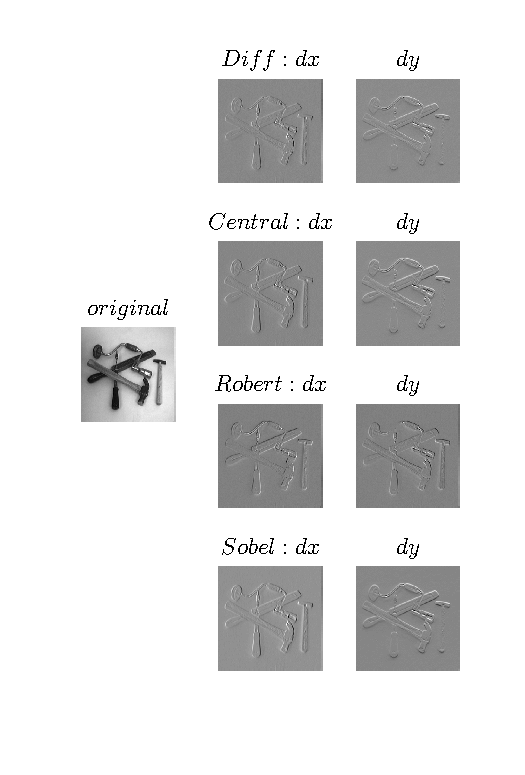
\includegraphics[width=0.8\textwidth]{q1}
 \caption{Gradient magnitude for different methods}
 \label{fig:q1}
\end{figure}

\paragraph{Question 1: 
What do you expect the results to look like and why? Compare the size of \texttt{dxtools} with the size of \texttt{tools}. Why are these sizes different?} 
Because we are using the \texttt{'valid'} option of the \texttt{conv2} function for the shape parameter which returns only those parts of the convolution that are computed without the zero-padded edges. The option \texttt{'same'} returns an image with the same size than the input but in which some parts have been computed using zero-padded edges.

\section{Point-wise thresholding of gradient magnitudes}

\begin{figure}[htbp]
 \centering
 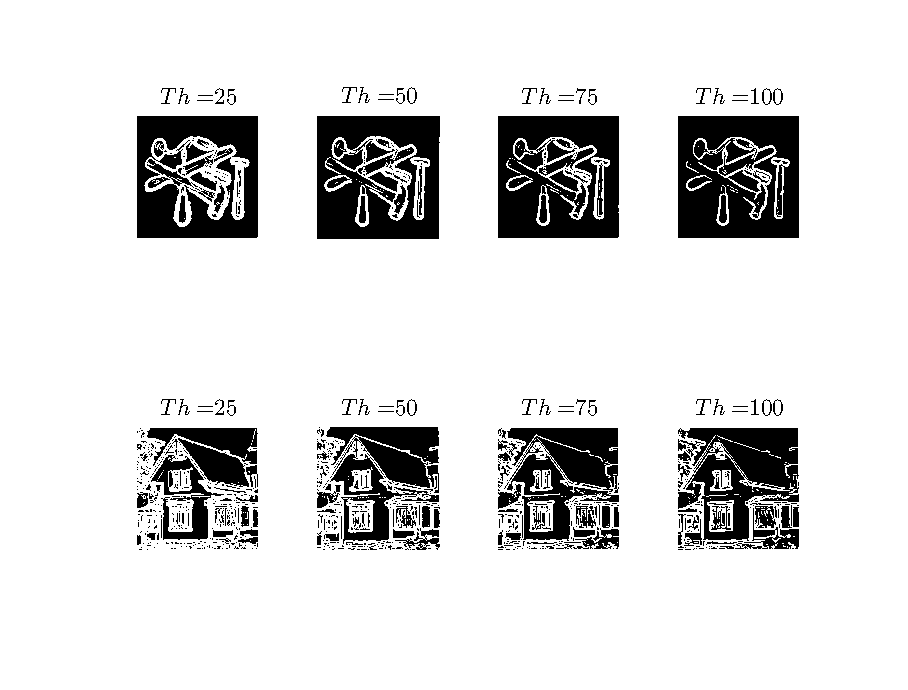
\includegraphics[width=\textwidth]{q2b}
 \caption{Thresholding gradient magnitude}
 \label{fig:q2b}
\end{figure}

\paragraph{Question 2:
it easy to find a threshold that results in thin edges? Explain why or why not!}
It is not easy because it depends on the amount of smoothing applied. If there is few smoothing many fake edges appear, if the smoothing is more smoothing the thickness of the edges increases.

\paragraph{Question 3: Does smoothing the image help to find edges?}
It helps defining which of the resulting edges are false or real edges, which is a matter of scale of what we want to find edges, i.e. edges of house or tree leafs.

\section{Computing differential geometry descriptors}

%% IMAGE POLYNOMIALS
\begin{figure}[htbp]
 \centering
 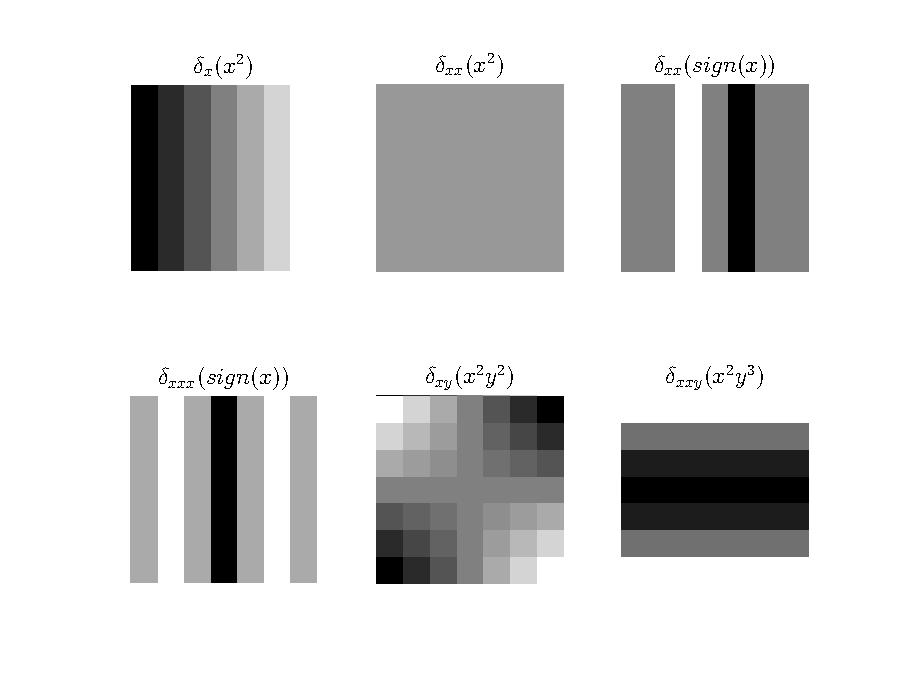
\includegraphics[width=\textwidth]{q4prev}
 \caption{Kernels tests}
 \label{fig:q4prev}
\end{figure}

%% ZERO CROSSINGS LVV HOUSE
\begin{figure}[htbp]
 \centering
 \includegraphics[width=\textwidth]{q45}
 \caption{Second order derivative zero-crossings and third order derivative sign.}
 \label{fig:q45}
\end{figure}

\paragraph{Question 4: What can you observe? Provide explanation based on the generated images.}
For smaller scale values, there appear many false edges, while for bigger values, the edges are distorted.

\paragraph{Question 5: Assemble the results of the experiment above into an illustrative collage
with the \texttt{subplot} command. Which are your observations and conclusions?}
The sign of the third derivative results in some areas around the edges which are wider for bigger scales.

\paragraph{Question 6: How can you use the response from \(\tilde{L}_{vv}\) to detect edges, and how can you improve the result by using \(\tilde{L}_{vvv}\)?}
The zero crossings of the second derivative are associated with points in which the gradient magnitude reaches local maxima or minima in the gradient direction, which can be edges or not. The edges are local maxima of this gradient, and can be classified by making use of the third derivative, which has to be of negative sign.

\section{Extraction of edge segments}

\begin{figure}[htbp]
 \centering
 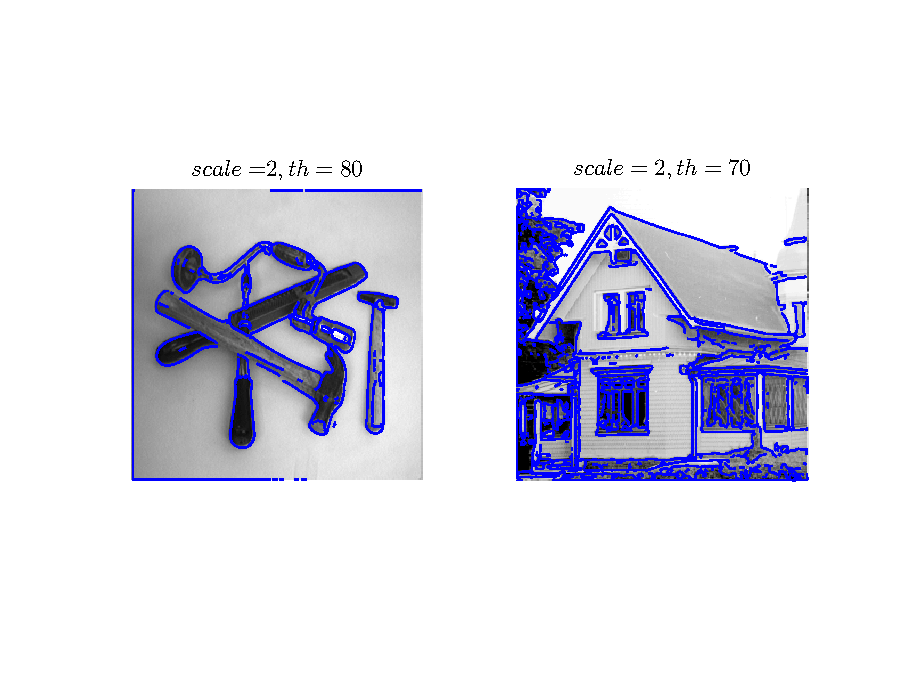
\includegraphics[width=\textwidth]{q6}
 \caption{Edges of \texttt{tools} and \texttt{house} images.}
 \label{fig:q45}
\end{figure}

\paragraph{Question 7: Present your best results obtained with \texttt{extractedge} for house and tools.}
Results shown in Figure \ref{fig:q45}.


\section{Hough transform}


%% Accumulator and original edges for triangle image
\begin{figure}[htbp]
 \centering
 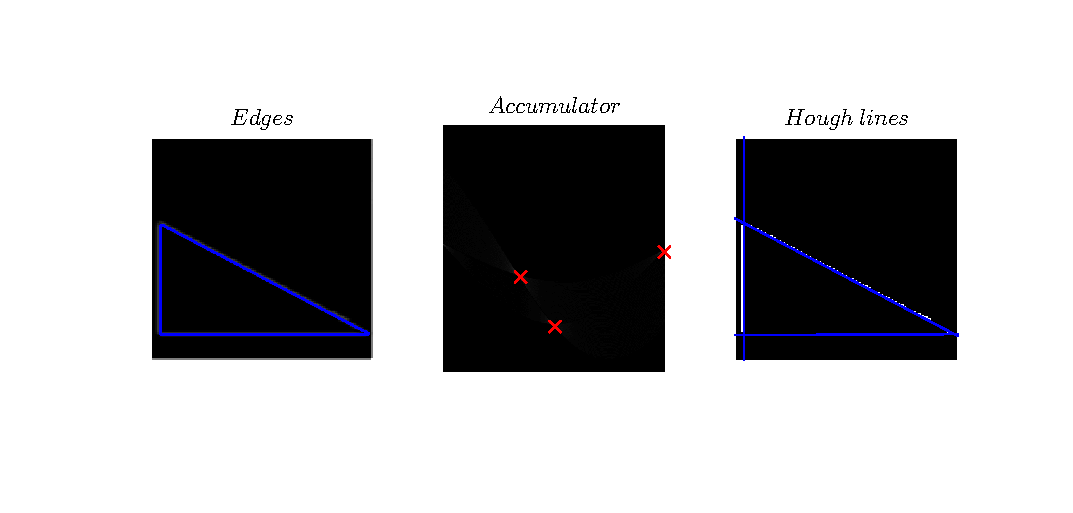
\includegraphics[width=\textwidth]{q8a}
 \caption{Gradient magnitude, Hough transform and Hough lines for \texttt{triangle} image}
 \label{fig:q8a}
\end{figure}

\begin{figure}[htbp]
 \centering
 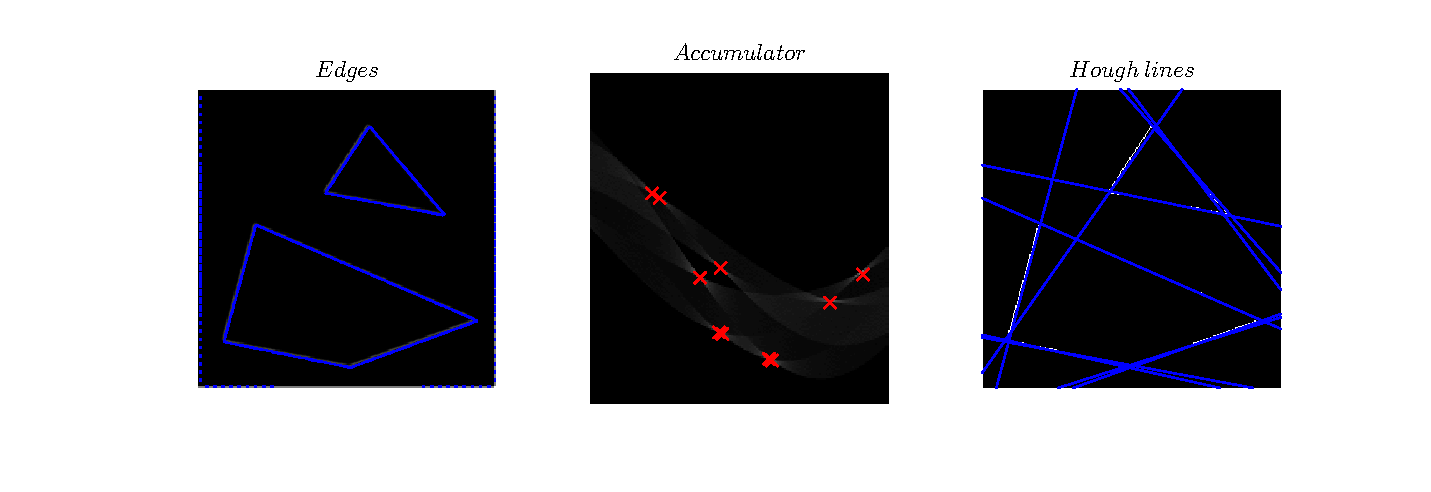
\includegraphics[width=\textwidth]{q8b}
 \caption{Gradient magnitude, Hough transform and Hough lines for \texttt{houghtest} image.}
 \label{fig:q8b}
\end{figure}

\begin{figure}[htbp]
 \centering
 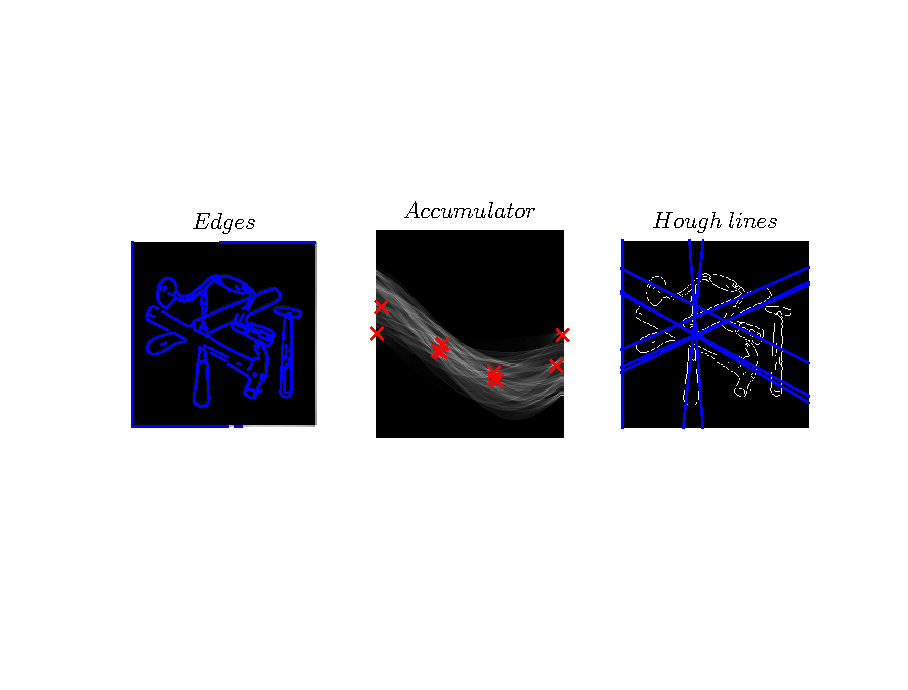
\includegraphics[width=\textwidth]{q8c}
 \caption{Gradient magnitude, Hough transform and Hough lines for \texttt{tools} image}
 \label{fig:q8c}
\end{figure}

\begin{figure}[htbp]
 \centering
 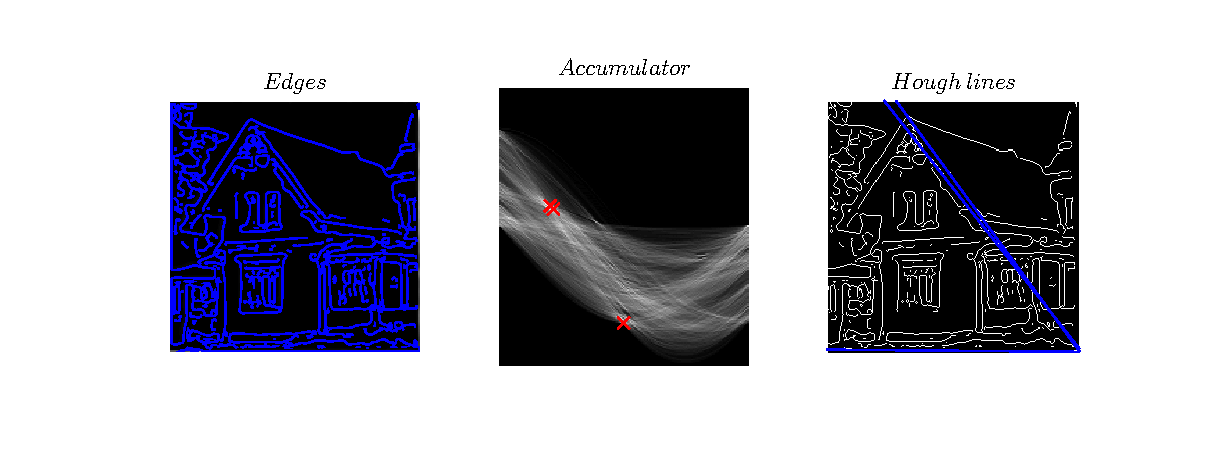
\includegraphics[width=\textwidth]{q8d}
 \caption{Gradient magnitude, Hough transform and Hough lines for \texttt{house} image.}
 \label{fig:q8d}
\end{figure}

\paragraph{Question 8: Identify the correspondences between the strongest peaks in the accumulator and line segments in the output image. Doing so convince yourself that the implementation is correct. Summarize the results of this study and print out on paper.} In \texttt{triangle} image, Figure \ref{fig:q8a}, the point at theta=90 and small rho is associated with the vertical line as represents the line y=rho. The point at theta=0 is associated with the horizontal line, x=rho, as sin(0)=0. In general, a line is associated with a point in the accumulator space by \(y=-\frac{1}{\tan\theta}x+\frac{\rho}{\sin\theta}\). Figure \ref{fig:q8b} shows the results for \texttt{houghtest} image and Figures \ref{fig:q8c} and \ref{fig:q8d} for \texttt{tools} and \texttt{house} respectively.

\paragraph{Question 9: How do the results and computational time depend on the number of cells in the accumulator?}
In one hand, the finer the grid in the accumulator (more cells), the more precise the lines associated to the chosen points, however, multiple points close to each other may give rise to multiple lines while they actually are the same line. In the other hand,  it implies more computational time, as has to compute the rho for more theta values for each edge point but the big difference is due to the size of the image.

\paragraph{Question 10: Choice of accumulator incrementation function. How do you propose to do this? Relate your answer to the different parts of the images.}
Accumulator increment can be instead of one, the gradient magnitude. This does not really help if the edge thickness in the magnitude of the gradient is too big. Using the gradient direction, we can assume that the orientation of the edge element is known (the gradient direction) so this element only votes for one bin in the accumulator, since theta is fixed by the edge orientation. However, gradient direction is not accurate enough so it is more interesting to put a range of angles around it so each curve generated by an edge element creates only a curve over some angles and not over all the theta space.



\end{document}
This is never printed
